\documentclass[11pt, oneside]{article}   	% use "amsart" instead of "article" for AMSLaTeX format
\usepackage{geometry}                		% See geometry.pdf to learn the layout options. There are lots.
\geometry{letterpaper}                   		% ... or a4paper or a5paper or ... 
%\geometry{landscape}                		% Activate for for rotated page geometry
%\usepackage[parfill]{parskip}    		% Activate to begin paragraphs with an empty line rather than an indent
\usepackage{graphicx}				% Use pdf, png, jpg, or eps� with pdflatex; use eps in DVI mode
								% TeX will automatically convert eps --> pdf in pdflatex		
\usepackage{amssymb}
\usepackage{parskip}

\graphicspath{{/Users/telliott_admin/Dropbox/Tex/png/}}

\title{Series}
%\author{The Author}
\date{}							% Activate to display a given date or no date

\begin{document}
\maketitle
%\section{}
%\subsection{}
\Large
The simplest series are arithmetic.  Each term differs from the previous one by addition or subtraction of a constant term.
\[ 1at,\ 2at,\ 2at,\ \cdots ,\ nat \]
One tricky point is that even though there are $n$ terms, there are only $n-1$ differences, hence subtracting the first from the last term gives $(n-1)at$.  And the reverse for finding the last from the number of terms and the difference $t$.  

Both the coefficient $a$ and the term $t$ can be factored out.  The sum of the series is
\[ S = at + a2t + a3t + \cdots  + ant \]
\[ S = at\sum_{k=1}^{n} k \]
We need the formula for the sum of the integers from $1$ to $n$
\[  1 + 2 + 3 + \cdots + n = ?  \]
There is a famous story about Gauss that (in the simplified version) he "saw" how to add the integers from $1$ to $100$ as two parallel sums
\[ \ \  1 + \ \ 2 + \ \ 3 + \cdots + 99 + 100 \]
\[ 100 + 99 + 98 + \cdots + 2 + 1 \]
Added together horizontally, these two series must equal twice the sum of $1-100$.  But notice that we have $n$ sums vertically, each of which is equal to $n+1$.  We see that
\[ 2S_n = n (n+1) \]
\[ S_n = \frac{1}{2} \ n (n+1) \]
Another proof follows the method of induction (see the writeup on induction).  Here is a striking "visual proof."
\begin{center}
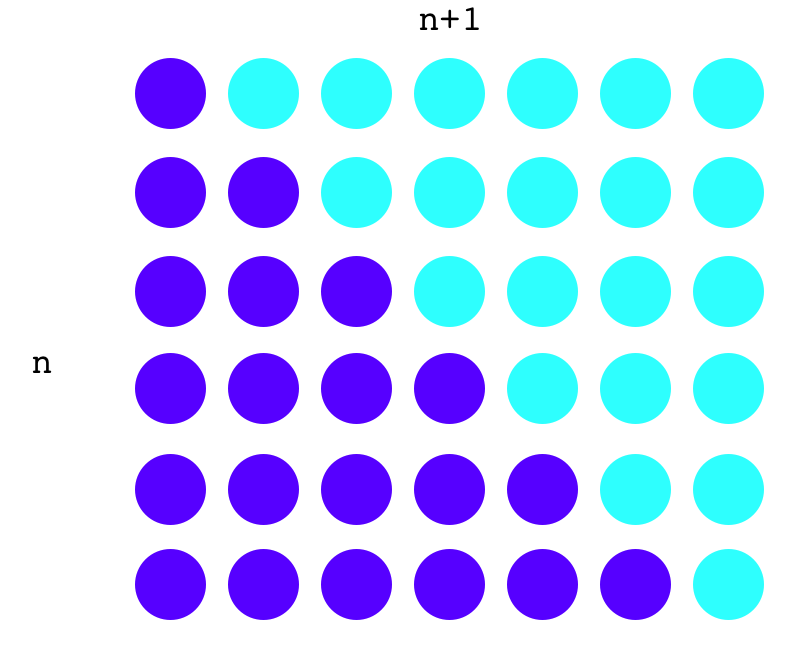
\includegraphics [scale=0.25] {sum_n.png}
\end{center}
There are $n$ rows and $n+1$ columns.  Either the dark blue or light blue circles by themselves are clearly equal to the sum we want.
\subsection*{Collapsing sum proof}
I want to show a fourth proof here.  It doesn't start very intuitively, but it uses a "collapsing sum", which is an important concept.
\[ (k+1)^2 = k^2 + 2k + 1 \]
\[ (k+1)^2 - k^2 = 2k + 1 \]
If we sum each term, we still have an equality
\[ \sum_{k=1}^n (k+1)^2 - \sum_{k=1}^n k^2  = \sum_{k=1}^n 2k + \sum_{k=1}^n 1 \]
The $lhs$ is a collapsing sum.  If we expand, it looks like this
\[lhs = [2^2 + 3^2 + 4^2 + \cdots + n^2 + (n+1)^2 ] - [1^2 + 2^2 + 3^2 + 4^2 + \cdots + n^2 ] \]
\[lhs = - 1^2 + 2^2 - 2^2 + 3^2 - 3^2 + 4^2 - 4^2 + \cdots + n^2 - n^2 + (n+1)^2 \]
All the terms disappear except
\[lhs = - 1^2 + (n+1)^2 \]
The right-hand side has what we want (almost).  The first term is
\[ \sum_{k=1}^n 2k = 2 \sum_{k=1}^n k = 2 S_n \]
And the second term is
\[ \sum_{k=1}^n 1 = n \]
Putting it all together we have
\[ 2 Sn + n = (n+1)^2 - 1 \]
\[ 2 Sn = n^2 + 2n + 1 - 1 - n = n^2 + n = n(n+1) \]
\[ Sn = \frac{1}{2} \ n(n+1) \]


\subsection*{Sum of Squares}
The sum of squares of the integers is given by
\[ S = \sum_{k=1}^{n} \ k^2 = 1^2 + 2^2 + 3^2 + \cdots + n^2 \]
\[ S = n(n+1)(2n+1)/6 \]

A proof for this one also follows the method of induction (see the writeup on induction).  For that method, one must guess the formula.

Here are two  approaches.  The first one is in Strang.  He says "the best place to start is a good guess".  So again:
\[ S = \sum_{k=1}^{n} \ k^2 \]
We guess
\[ S_n = \frac{1}{3} n^3 \]
To test it, check whether the difference is $n^2$ as it should be:
\[ S_{n} - S_{n-1} = \frac{1}{3} n^3 - \frac{1}{3} (n-1)^3 \]
Now
\[ (n-1)^2 = n^2 - 2n + 1 \]
\[ (n-1)^3 = (n-1)(n^2 - 2n + 1) \]
\[ = n^3 - 3 n^2 + 3 n - 1\]
So
\[ S_{n} - S_{n-1} = \frac{1}{3} (n^3 - n^3 + 3 n^2 - 3 n + 1) \]
We see that our guess is off by
\[ \frac{1}{3} (3 n^2 - 3 n + 1) \]
\[ = n^2 - n + \frac{1}{3} \] 
Strang says:  the guess needs \emph{correction terms}.  
To cancel $1/3$ in the difference, subtract $n/3$ from the sum.  And to add back $n$ in the difference, add back $1 + 2 + \dots + n(n+1)/2$ to the sum.  Our new guess is

\[ S_n =  \frac{1}{3} n^3 + \frac{n(n+1)}{2} - \frac{n}{3} \]
\[ = \frac{n}{6} (2n^2 + 3(n+1) - 2) \]
\[ =  \frac{n}{6} (2n + 1)(n + 1) \]
\[ = \frac{n(n+1)(2n+1)}{6} \]
which may be easier to remember as
\[ S_n = \frac{n(n+1)}{2} \times \frac{2n + 1}{3} \]
If you check this as we did before, you will find that it is correct.

The second is an algebraic proof which uses a "collapsing sum."

\[ (k+1)^3 = k^3 + 3k^2 + 3k + 1 \]
\[ (k+1)^3 - k^3 = 3k^2 + 3k + 1 \]
\[ \sum_{k=1}^n (k+1)^3 - \sum_{k=1}^n k^3 = \sum_{k=1}^n 3k^2 + \sum_{k=1}^n 3k + \sum_{k=1}^n 1 \]
Looks kind of familiar!  The $lhs$ collapses to just two terms
\[ lhs = (n+1)^3 - 1 \]
The right hand side has what we want (almost)
\[ rhs = \sum_{k=1}^n 3k^2 + \sum_{k=1}^n 3k + \sum_{k=1}^n 1 \]
\[ rhs = 3S_{n^2} + 3S_n + n \]
\[ 3S_{n^2} = (n+1)^3 - 1 - n - \frac{3}{2} n(n+1) \]
\[ 3S_{n^2} = (n+1)^3 - (n + 1) - \frac{3}{2} n(n+1) \]
\[ 3S_{n^2} = (n+1) \ [ \ (n+1)^2 - 1 - \frac{3}{2} n \ ]\]
\[ 3S_{n^2} = \frac{1}{2} \ (n+1) \ [ \ 2(n+1)^2 - 2 - 3n \ ]\]
\[ S_{n^2} = \frac{1}{6} \ (n+1) \ [ \ 2n^2 + 4n + 2 - 2 - 3n \ ]\]
\[ S_{n^2} = \frac{1}{6} \ (n+1) \ [ \ 2n^2 + n \ ]\]
\[ S_{n^2} = \frac{1}{6} \ (n+1) \ (n) \ (2n + 1) \]
\[ S_{n^2} = \frac{(n) \ (n+1) \ (2n + 1)}{6}  \]


\subsection*{Geometric Series}
The geometric series is usually given like this:
\[ T = a + ar + ar^2 + ar^3 \cdots + ar^{n-1} = \sum_{k=0}^{n-1} ar^k \]
where $a$ is the first term and $r$ is the common ratio.  Again, the sum goes to the $n-1$ term because we have started with the $k=0$, so there are $n$ terms in whole sum.

Each term is different by a factor of $r$ from the preceding one.  When the emphasis is on arithmetic including an $a$ helps make the problem harder, but it is really irrelevant.  The constant $a$ can be factored out of each term so that 
\[ T = a \ \sum_{k=0}^{n-1} r^k = aS  \]

Let's look at the simpler version
\[ S = 1 + r + r^2 + r^3 \cdots + r^{n-1} = \sum_{k=0}^{n-1} r^k \]
To solve this, note that 
\[ rS = r + r^2 + r^3 \cdots + r^{n-1} + r^n \]
\[ S - rS = 1 - r^n \]
\[ S = (1 - r^n)/(1-r) \]
Be careful, because the formula includes $r^n$ whereas the last term actually given is $r^{n-1}$.

\end{document}  